This section will give a broad overview of the whole System under development. It will explain how the System interacts with external systems and introduce its main functionality.

It will also describe the end users and the functionalities of the System reserved to them, detailing all the informations relevant to clarify their needs.

At last it will present the constraints and assumptions made for the System under development.

\subsection{Product Perspective}

This System will be implemented ex-novo to support all the functionalities required by the \textit{PowerEnJoy Car-Sharing} Service.

The System will be able to communicate with all the involved external systems, such as the Database,in which all the information are stored and can be modified by the System, the Banking System, needed to perform the monetary transactions, the Mailing System, which will forward the emails generated by the System, and the Mapping System, which is used in particular to show the GPS position of Cars, Users and Parking Areas on a map, check for existing addresses, and get the exact desired position in a specified address. The System will adopt the HTTP(S) protocol to communicate with the above specified systems managing the interactions through a set of shared protocols and APIs.
\smallskip

End users will access the System functionalities through an Internet connection, using the User intended interface of the System, the Application. Hence, the System should also be able to implement the Application Layer of the Internet Protocol Suite.
Users will communicate their position to the System using the GPS coordinates in order to unlock the previously reserved Car.
\smallskip

At last, the System should be able to communicate with the wide variety of sensors placed inside the Cars, in order to know, in every moment, their position, the status of their battery, their possible damages, their plugged status and the number of seats occupied. 

\subsubsection{Class Diagram}
\begin{figure}[h]
\centering
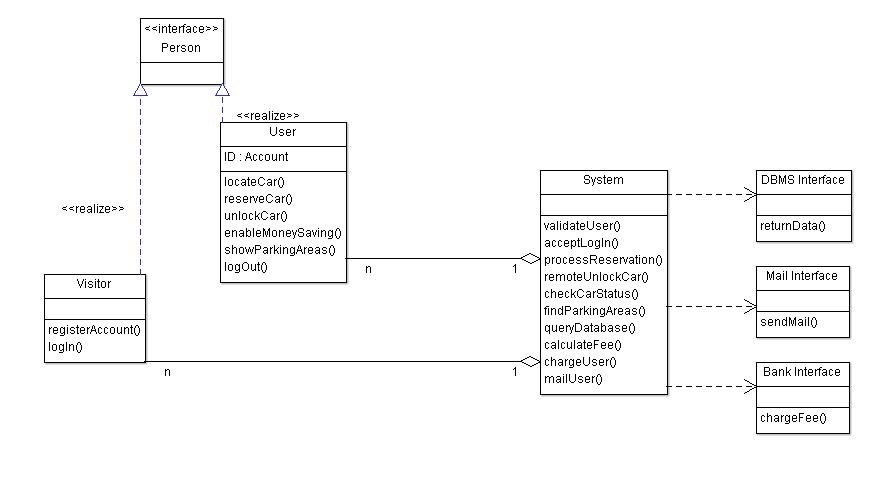
\includegraphics[width=\linewidth,keepaspectratio]{../Diagrams/CD/Class_Diagram.png}
\caption{Class Diagram}
\end{figure}
\FloatBarrier

\subsubsection{Statechart}
\begin{figure}[h]
\centering
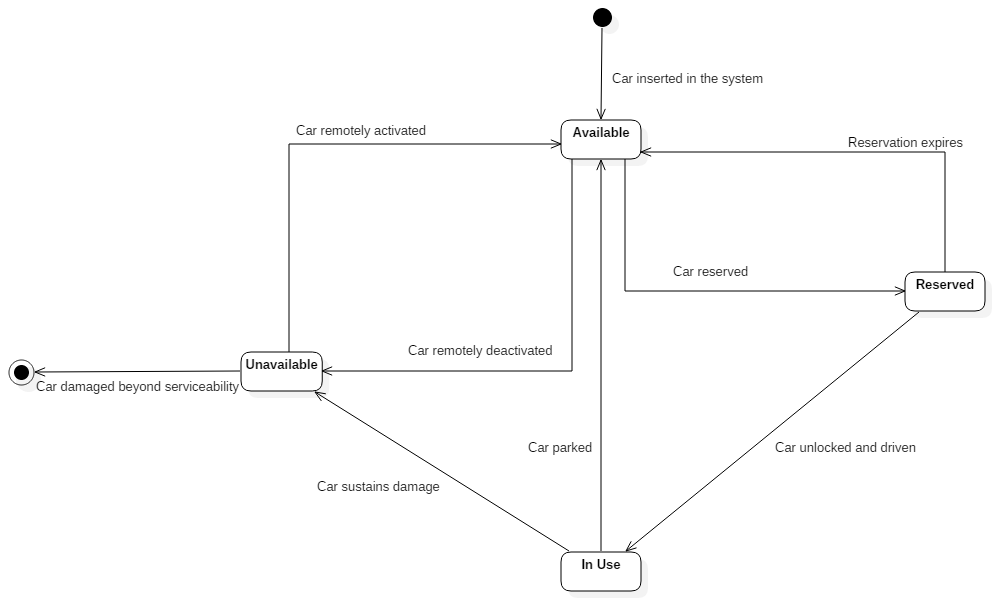
\includegraphics[width=\linewidth,keepaspectratio]{../Diagrams/SCD/SCD_Car.png}
\caption{Statechart diagram of Car}
\end{figure}
\FloatBarrier

\subsection{Product Functions}
Using the the Application, the User will be able to register an account in the System, log in the System and so finally access the System functionalities dedicated to users. The User can now locate all the Cars, whose state is \textit{Available}, specifying a desired address or asking the System to locate him/her through the GPS coordinates.\\
The Mapping System is now asked to check for the existence of the specified address or locate the User's position, showing on the map all the \textit{Available} Cars, together with their intrinsic information, in a distance range specified by the System. 
\smallskip

The User can now decide to reserve a Car, from this moment a one hour countdown starts during which the User will be able to unlock his/her reserved Car.
The User can unlock the Car asking the System to locate him/her and if the Mapping System verifies that the User is in a specified distance range from the Car, the Car is unlocked and the User can now enter and drive it. If the User doesn't unlock the Car during the previous specified time period, the System cancels the reservation, sets the Car status as \textit{Available} and communicates to the Banking System the application of a fee.
\smallskip


At the end of the ride, the System, basing on the time usage period of the Car, and on bad or good behaviors preset by the System will evaluate the Fee and notify and the Banking System of the total amount to charge to the User's credit card.


%TODO format requirements
\newcounter{RequirementsCounter}
\stepcounter{RequirementsCounter}

%\begin{center}
%  \begin{longtable}{|p{.2\textwidth}|p{.12\textwidth}|p{.58\textwidth}|}
%    \hline
%    \textbf{Goal} & \textbf{Priority} & \textbf{Function} \\ \hline
%    Registration & High & Allows a Visitor to register their credentials, becoming a User \\ \hline
%    Login & High & Lets a User access the system \\ \hline
%    Find Nearby Cars & ? & Shows Available Cars in a location \\ \hline
%    Reservation & ? & Allows a user to set a nearby Car as Reserved \\ \hline
%    Proximity Unlock & ? & Unlocks the car when the User who Reserved it is close \\ \hline
%  \end{longtable}
%\end{center}

\subsection{User Classes and Characteristics}
\begin{center}
  \begin{tabular}{|p{.2\textwidth}|p{.39\textwidth}|p{.39\textwidth}|}
    \hline
    \textbf{Name} & \textbf{Description} & \textbf{Actions} \\ \hline
    Visitor & A person who would like to register an account to access the System functionalities. & Can perform the registration and activation of the account. Successively he can log in the System becoming a User.\\\hline
    User & Someone who is registered in the System and can access its functionalities & Can locate, reserve and drive Cars. Will be charged for the use of the Cars. \\ \hline
    \end{tabular}
\end{center}
\vspace{5mm}
External access to the Database provided to Employees and Administrators is under the responsibility and the regulations of the Company and is not managed by this System.


\subsection{Constraints}
\subsubsection{Hardware Constraints}\label{OE}
The device used by the User should be able to establish an internet connection to the System using the Application. In addition, in order to perform the localization, reservation and unlocking of a Car the device must have installed a working GPS module. 

\subsubsection{Design and Implementation Constraints}
The system will employ the HTTP(S) protocol in order to communicate with the Database, the external systems, and with the User through the Application. 

\subsection{Assumptions and Dependencies}
\begin{enumerate}
	\item The User can only have one Account at time.
	\item The Company can decide at any time to block an User from accessing to the System (f.e. for improper behavior, unpaid bill, ...). It will be done by employees or Administrators.
	\item The User always provides real correct data in his/her registration form.
	\item The Database in which the Cars, Parking Areas, Charging Areas, Users,etc, are stored, is owned and managed from the Company (and not by this System), which is responsible for its security, reliability and availability. Our System is provided by the Company with read/write access to this Database.
	\item The Company is responsible for the employees and their actions.
	\item The Car has a set of sensors that can detect, in every moment, its position, the status of its battery, the status of the engine, its damages, the connection of its plug to an electrical socket and the number of seats occupied. We assume that these sensors won't ever break down and that their measures are always correct.
	\item The Car GPS always detects its position with absolute precision.
	\item The User always enters the Car when he/she unlocks its doors.	
	\item After a Car is Plugged, it will not be maliciously unplugged by the User himself/herself or by other people.
	\item After the doors of the cars are unlocked by the User, he/she always enters the Car, ignites the engine and leave the Parking Area.
	\item An User can park/stop the Car everywhere and leave the Car at anytime. However, the system will end the ride (i.e. stop charging the User) only if he/she turns the engine off inside a Parking Area.
	\item When the User gets at least two Passengers, the corresponding discount on the User's fee will be applied only if the passengers stay together in the Car for more than 3 minutes. 
	\item When a User will park the Car inside a Parking Area, it will always correctly use one and only one free slot.
	\item As soon as the Car battery status gets below 20\% of the full capacity AND the Car isn't in a Charging Area AND the Car Status isn't \textit{In Use} OR \textit{Plugged}, there's always an Employee that immediately reaches the Car and recharges it on site; in the meanwhile the Car status is \textit{Unavailable}.	
	\item When the Car is \textit{In Use} and the battery charge level reaches the 0\% of the full capacity the Car stops working and is immediately set as \textit{Unavailable}.
	If the Car status is \textit{Unavailable}, the Car will be reached by an Employee to consider if the Car needs to be taken in the Company's workshop for repairs or just needs to be recharged.
	\item The Car has the ability to detect if it has been damaged. 
	\item If the Car status is \textit{In Use} when a \textit{Minor damage} is detected, the Car status will be set to \textit{Unavailable} at the end of the ride; if a \textit{Major damage} is detected the Car status is immediately set to \textit{Unavailable}. In both cases an employee will reach the car and cope with the damages, deciding if the Car can be immediately used again (sets it to \textit{Available}) or should be moved to the Company's workshop and/or if the User should pay for the damages. 
	\item A car which is \textit{Available} or \textit{Plugged} can be set as \textit{Unavailable} in every moment by an Employee. This is done through another Company's System as it is not provided in this System.
	\item A car which is \textit{Unavailable} can be set to \textit{Available} in every moment by an Employee.  This is done through another Company's System and it is not provided in this System.
	\item If the Car has been left out of a Parking Area there will always be an employee which immediately reaches it, recharges it and move it to a Charging Area. 
	\item Every fine received by the Company for improper use of the Car will be managed by the Company.
	
\end{enumerate}

\clearpage